\chapter{Local search}

\begin{description}
    \item[Local search] \marginnote{Local search}
        Starting from an initial state, iteratively improves it by making local moves in a neighborhood.

        Useful when the path to reach the solution is not important (i.e. no optimality).

    \item[Neighborhood] \marginnote{Neighborhood}
        Given a set of states $\mathcal{S}$, a neighborhood is a function:
        \[ \mathcal{N}: S \rightarrow 2^\mathcal{S} \]
        In other words, for each $s \in \mathcal{S}$, $\mathcal{N}(s) \subseteq \mathcal{S}$.

        \begin{example}[Travelling salesman problem]
            Problem: find an Hamiltonian tour of minimum cost in an undirected graph.
            
            A possible neighborhood of a state applies the $k$-exchange that guarantees to maintain an Hamiltonian tour.
            \begin{figure}[ht]
                \begin{subfigure}{.5\textwidth}
                    \centering
                    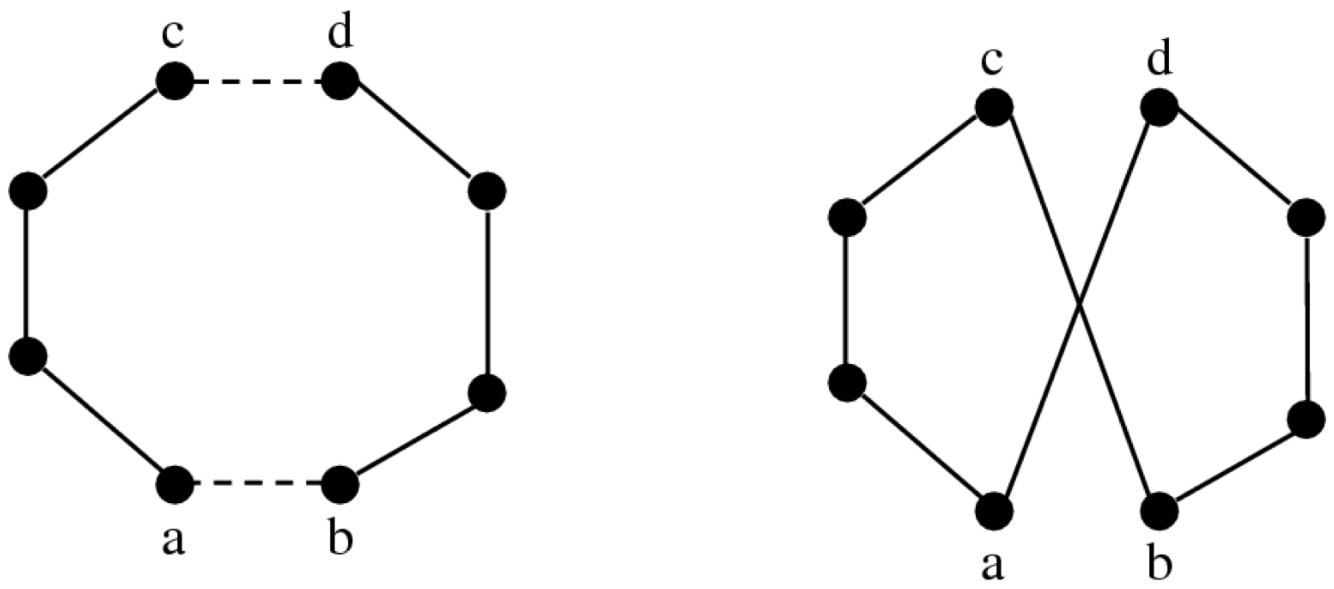
\includegraphics[width=.70\linewidth]{img/tsp_2-exchange.png}
                    \caption{2-exchange}
                \end{subfigure}%
                \begin{subfigure}{.5\textwidth}
                    \centering
                    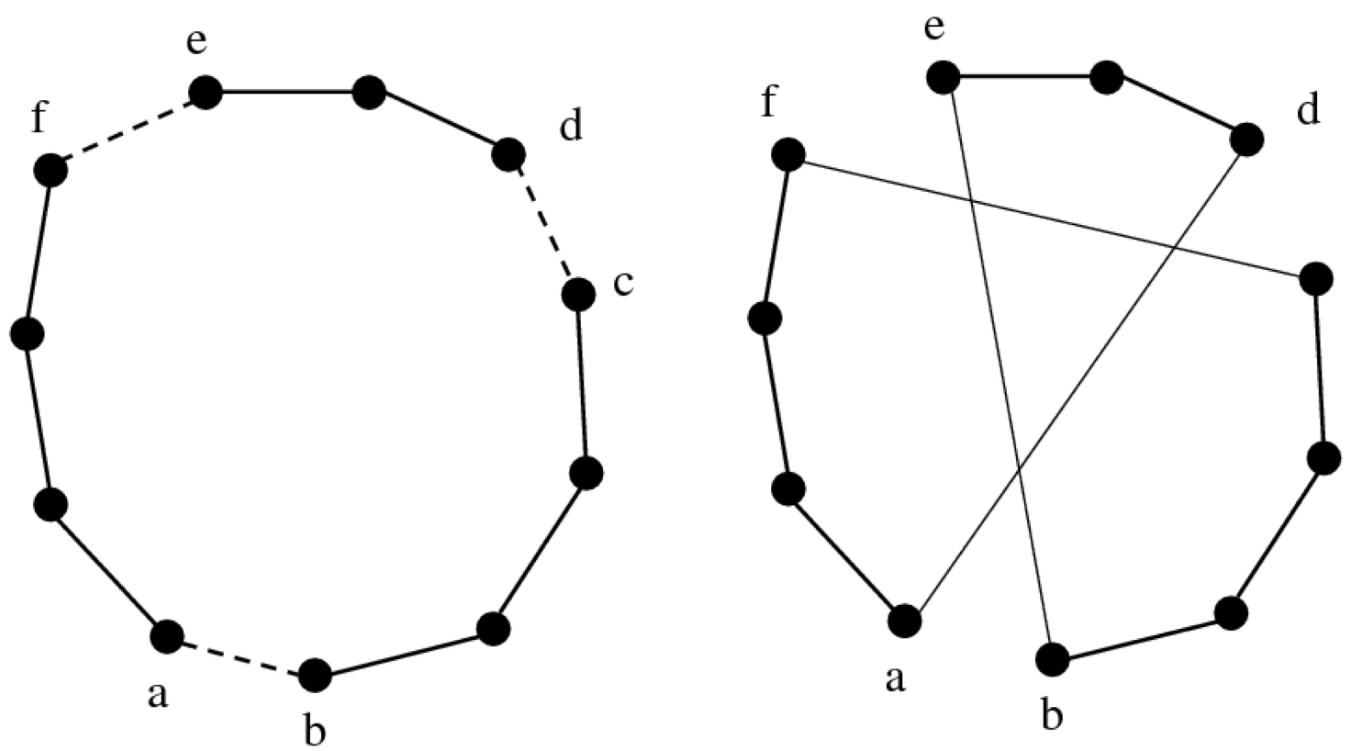
\includegraphics[width=.70\linewidth]{img/tsp_3-exchange.png}
                    \caption{3-exchange}
                \end{subfigure}
            \end{figure}
        \end{example}

        
    \item[Local optima]
    Given an evaluation function $f$,
    a local optima (maximization case) is a state $s$ such that:
    \[ \forall s' \in \mathcal{N}(s): f(s) \geq f(s') \]

    \item[Global optima]
        Given an evaluation function $f$,
        a global optima (maximization case) is a state $s_\text{opt}$ such that:
        \[ \forall s \in \mathcal{S}: f(s_\text{opt}) \geq f(s) \]

        Note: a larger neighborhood usually allows to obtain better solutions.

    \item[Plateau]
        Flat area of the evaluation function.

    \item[Ridges]
        Higher area of the evaluation function that is not directly reachable.
\end{description}



\section{Iterative improvement (hill climbing)}
\marginnote{Iterative improvement (hill climbing)}
Algorithm that only performs moves that improve the current solution.

It does not keep track of the explored states (i.e. may return in a previously visited state) and 
stops after reaching a local optima.

\begin{algorithm}
\caption{Iterative improvement}
\begin{lstlisting}
def iterativeImprovement(problem):
    s = problem.initial_state
    while noImprovement():
        s = bestOf(problem.neighborhood(s))
\end{lstlisting}
\end{algorithm}



\section{Meta heuristics}
\marginnote{Meta heuristics}
Methods that aim to improve the final solution.
Can be seen as a search process over graphs:
\begin{descriptionlist}
    \item[Neighborhood graph] The search space topology.
    \item[Search graph] The explored space.
\end{descriptionlist}
\begin{figure}[ht]
    \begin{subfigure}{.5\textwidth}
        \centering
        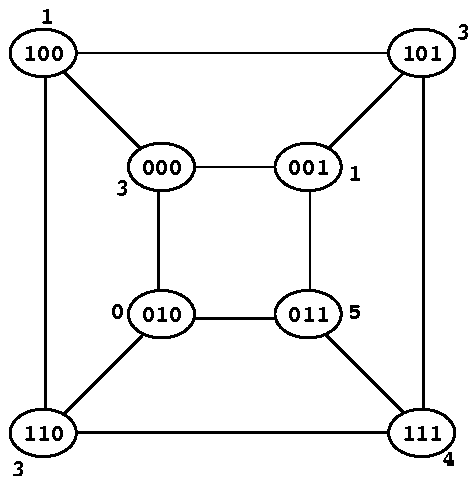
\includegraphics[width=.55\linewidth]{img/_local_search_neigh_graph.pdf}
        \caption{Neighborhood graph}
    \end{subfigure}%
    \begin{subfigure}{.5\textwidth}
        \centering
        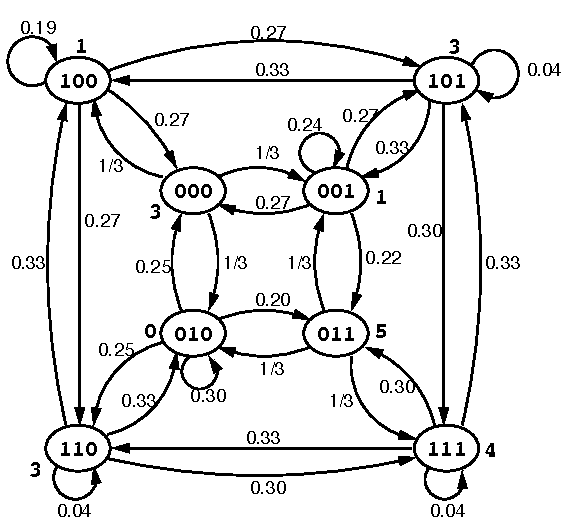
\includegraphics[width=.60\linewidth]{img/_local_search_search_graph.pdf}
        \caption{Search graph. Edges are probabilities}
    \end{subfigure}
\end{figure}

Meta heuristics finds a balance between:
\begin{descriptionlist}
    \item[Intensification] \marginnote{Intensification}
        Look for moves near the neighborhood.
    \item[Diversification] \marginnote{Diversification}
        Look for moves somewhere else.
\end{descriptionlist}

Different termination criteria can be used with meta heuristics:
\begin{itemize}
    \item Time constraints.
    \item Iterations limit.
    \item Absence of improving moves (stagnation).
\end{itemize}


\subsection{Simulated annealing}
\marginnote{Simulated annealing}
Occasionally allow moves that worsen the current solution.
The probability of this to happen is:
\[
    \frac{e^{f(s) - f(s')}}{T}
\]
where $s$ is the current state, $s'$ is the next move and $T$ is the temperature.
The temperature is updated at each iteration and can be:
\begin{descriptionlist}
    \item[Logarithmic] $T_{k+1} = \Gamma / \log(k + k_0) $
    \item[Geometric] $T_{k+1} = \alpha T_k$, where $\alpha \in\, ]0, 1[$
    \item[Non-monotonic] $T$ is alternatively decreased (intensification) and increased (diversification).
\end{descriptionlist}

\begin{algorithm}
\caption{Meta heuristics -- Simulated annealing}
\begin{lstlisting}[mathescape=true]
    def simulatedAnnealing(problem, T0):
        s = problem.initial_state
        T, k = T0, 0
        while not terminationConditions():
            s_next = randomOf(problem.neighborhood(s))
            if (problem.f(s_next) > problem.f(s) or
               downHillWithProbability($e^{\texttt{problem.f(\texttt{s}) - problem.f(s\_next)}} \texttt{/ T}$)):
                s = s_next
            k += 1
            update(T, k)
\end{lstlisting}
\end{algorithm}


\subsection{Tabu search}
\marginnote{Tabu search}
Keep track of the last $n$ explored solutions in a tabu list and forbid them.
Allows to escape from local optima and cycles.

Since keeping track of the visited solutions is inefficient, 
moves can be stored instead but, with this approach, some still not visited solutions may be cut off.
\textbf{Aspiration criteria} can be used to allow forbidden moves in the tabu list to be evaluated.

\begin{algorithm}
\caption{Meta heuristics -- Tabu search}
\begin{lstlisting}[mathescape=true]
    def tabuSearch(problem, T0):
        s = problem.initial_state
        tabu_list = [] # limited to n elements
        T, k = T0, 0
        while not terminationConditions():
            allowed_s = $\{ s' \in \mathcal{N}(s): s' \notin \texttt{tabu\_list} \texttt{ or } \texttt{aspiration condition satisfied} \}$
            s = bestOf(allowed_s)
            updateTabuListAndAspirationConditions()
            k += 1
            update(T, k)
\end{lstlisting}
\end{algorithm}


\subsection{Iterated local search}
\marginnote{Iterated local search}
Based on two steps:
\begin{descriptionlist}
    \item[Subsidiary local search steps] Efficiently reach a local optima (intensification).
    \item[Perturbation steps] Escape from a local optima (diversification).
\end{descriptionlist}
In addition, an acceptance criterion controls the two steps.

\begin{algorithm}
\caption{Meta heuristics -- Iterated local search}
\begin{lstlisting}[mathescape=true]
    def tabuSearch(problem):
        s = localSearch(problem.initial_state)
        while not terminationConditions():
            s_perturbation = perturbation(s, history)
            s_local = localSearch(s_perturbation)
            s = acceptanceCriterion(s, s_local, history)
\end{lstlisting}
\end{algorithm}


\subsection{Population based (genetic algorithm)}
\marginnote{Population based (genetic algorithm)}

Population based meta heuristics are built on the following concepts:
\begin{descriptionlist}
    \item[Adaptation] Organisms are suited to their environment.
    \item[Inheritance] Offspring resemble their parents.
    \item[Natural selection] Fit organisms have many offspring, others become extinct.
\end{descriptionlist}

\begin{table}[ht]
    \centering
    \begin{tabular}{c | c}
        \textbf{Biology} & \textbf{Artificial intelligence} \\
        \hline
        Individuals & Possible solution \\
        Fitness & Quality \\
        Environment & Problem \\
    \end{tabular}
    \caption{Biological evolution metaphors}
\end{table}

% The evolutionary cycle of a genetic algorithm has the following steps:
% \begin{descriptionlist}
%     \item[Recombination] Combine the genetic material of the parents.
%     \item[Mutation] Introduce variability.
%     \item[Selection] Selection of the parents.
%     \item[Replacement/Insertion] Define the new population.
% \end{descriptionlist}
The following terminology will be used:
\begin{descriptionlist}
    \item[Population] Set of individuals (solutions).
    \item[Genotypes] Individuals of a population.
    \item[Genes] Units of chromosomes.
    \item[Alleles] Domain of values of a gene.
\end{descriptionlist}

\begin{figure}[ht]
    \centering
    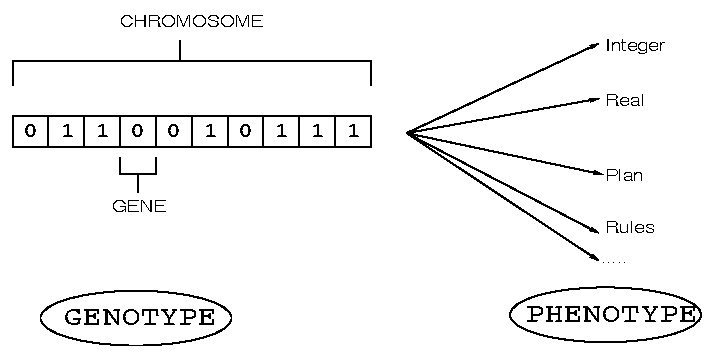
\includegraphics[width=0.5\textwidth]{img/_genetic_terminology.pdf}
    \caption{}
\end{figure}


Genetic operators are:
\begin{descriptionlist}
    \item[Recombination/Crossover] 
        Cross-combination of two chromosomes.
        \begin{center}
            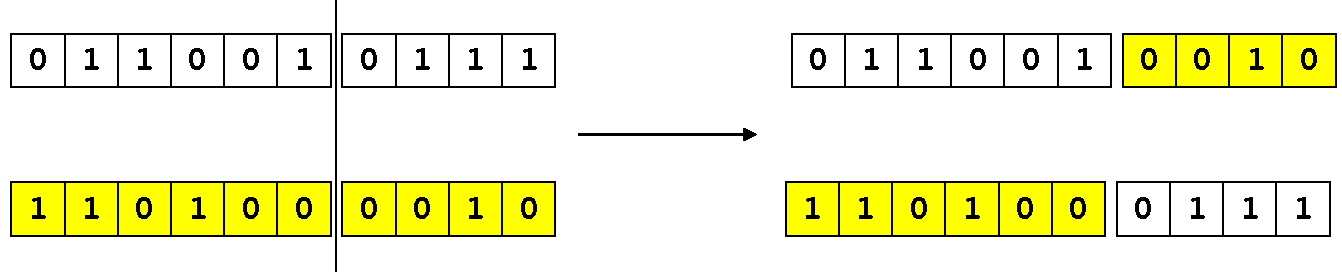
\includegraphics[width=0.5\textwidth]{img/_genetic_crossover.pdf}
        \end{center}
    \item[Mutation] 
        Random modification of genes.
        \begin{center}
            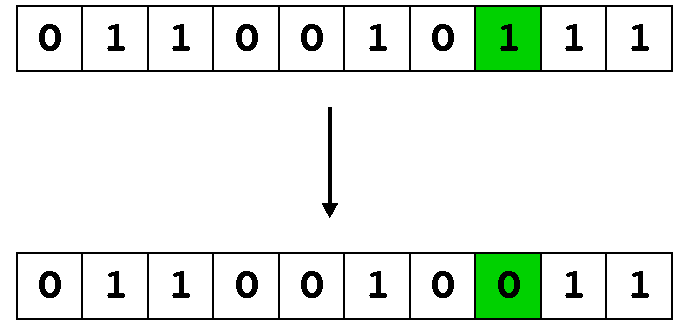
\includegraphics[width=0.2\textwidth]{img/_genetic_mutation.pdf}
        \end{center}
    \item[Proportional selection] 
        Probability of a individual to be chosen as parent of the next offspring. 
        Depends on the fitness.
    \item[Generational replacement] 
        Create the new generation. Possibile approaches are:
        \begin{itemize}
            \item Completely replace the old generation with the new one.
            \item Keep the best $n$ individual from the new and old population.
        \end{itemize}
\end{descriptionlist}

\begin{example}[Real-valued genetic operators]
    Solution $x \in [a, b]$ with $a, b \in \mathbb{R}$.
    \begin{descriptionlist}
        \item[Mutation] Random perturbation: $x \rightarrow x \pm \delta$, as long as $x \pm \delta \in [a, b]$.
        \item[Crossover] Linear combination: $x = \lambda_1 y_1 + \lambda_2 y_2$, as long as $x \in [a, b]$.
    \end{descriptionlist}
\end{example}

\begin{example}[Permutation genetic operators]
    Solution $x = (x_1, \dots, x_n)$ is a permutation of $(1, \dots, n)$.
    \begin{descriptionlist}
        \item[Mutation] Random exchange of two elements at index $i$ and $j$, with $i \neq j$.
        \item[Crossover] Crossover avoiding repetitions.
    \end{descriptionlist}
\end{example}

\begin{figure}[ht]
    \centering
    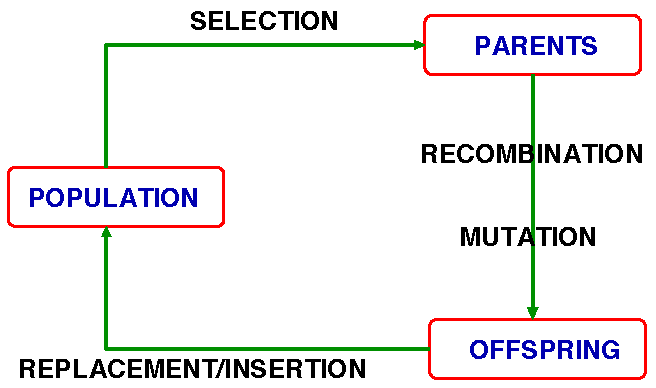
\includegraphics[width=0.4\textwidth]{img/_genetic_cycle.pdf}
    \caption{Evolutionary cycle}
\end{figure}

\begin{algorithm}
\caption{Meta heuristics -- Genetic algorithm}
\begin{lstlisting}[mathescape=true]
    def geneticAlgorithm(problem):
        population = problem.initPopulation()
        evaluate(population)
        while not terminationConditions():
            offspring = []
            while not offspringComplete(offspring):
                p1, p2 = selectParents(population)
                new_individual = crossover(p1, p2)
                new_individual = mutation(new_individual)
                offspring.append(new_individual)
            population = offspring
            evaluate(population)
\end{lstlisting}
\end{algorithm}